\section{Code generation pattern}
\label{sec:codegen}
%\subsection{Transformation pattern}
%todo: describe the pattern

%Transformation from State machine to fUML (classes, attributes, methods)
%\lipsum[1]

\subsection{Assumption}
%todo: give some assumptions on code generation such as functions to create methods, attriutes, classes
Assuming that we want to generate from the state machine to an object oriented programming language $ActLang$, which is a C++-like and supports multi-threading as following functions and resource control as mutexes.
\begin{itemize}
	%\item $genClass(n, generals, itfs)$ creates a class with its name, parent class set, and implemented interfaces as \ti{n}, \ti{generals}, and \ti{itfs}.
	
	%\item $genMtd(n, c, type, params)$ creates a method $m$ with its name as $n$ inside the class $c$, its return type as $type$, and $params$ as its parameter set.
	
	%\item $genAttr(n, c, type, multiplicity)$ creates an attribute named $n$ in the class $c$ and typed by $type$. The create attribute is an array if $multiplicity > 1$, otherwise a simple attribute.
	
	%\item $genEnum(n)$ and $genEnumLit(enum, n)$ create an enumeration and its enumeration literal, respectively.
	
	%\item $genBody(m, body)$ adds a body to a method. The body is a string which contains a list of statements.
	
	%\item $createParalle(t, seg)$ generates a mechanism which allows the segment code $seg$ run in a thread $t$. Similarly, $genWait(t), genJoin(t)$.
	
	\item A mutex has three methods $lock$, $unlock$, and $wait$, which automatically unlock the mutex and waits until it receives a signal.  
	
	%\item $synchronize(seg)$ generates a mechanism which allows the segment code $seg$ run safely (can be either based on \ti{POSIX pthread} or \ti{Java synchronize} mechanism).
	
	%\item $toString(stts)$ is used to convert a list of statements $stts$ into a readable string which can be add to a method as its body.
	
	%\item Concatenation of two strings $str1$ and $str2$ is concisely described as $str1 + str2$.
	
	%\item \ti{WHILE}, \ti{FOR} \ti{IF}, \ti{ELSE} are symbols representing while and for loops, if and else statements.
	
	\item \ti{FORK(func)} creates a thread (lightweight process) associated with the function/method \ti{func} and \ti{JOIN(theThread)} waits until the method associated with the thread \ti{theThread} completes.
\end{itemize} 

\subsection{State transformation}
Suppose that we want to generate a state machine $sm$ whose states are listed by $lstates$. A common state interface $IState$ is created. The interface contains three methods, namely, \ti{entry}, \ti{exit}, and \ti{doActivity} corresponding to three state actions, respectively. To preserve the hierarchy of composite states, the interface also has two attributes called \ti{activeStates} and \ti{previousStates} referring to active sub-states \ti{actives} , previous active sub-states \ti{previousStates} in case of the presence of history states, and a list of deferred event identifiers.

Each UML state is transformed into an instance of the interface associated with a state ID (which is a child element of an enumeration) inside the active class $C$. When initialization, each instance refers its methods to the actual methods implemented in $C$. In C++, this referring is done by using the powerful mechanism function pointer. In other object-oriented languages such as Java, this is done with anonymous sub-classes of the interface. Listing \ref{lst:IStateCpp} and \ref{lst:IStateJava} show the interface and its instances associated with the states of the state machine in C++ and Java, respectively, in which S0 is one of $lstates$. \ti{NUM\_STATES} is the number of states in the state machine. The actions of the states are implemented in the active class $C$ and named depending on the name of the states. In the following sections, we only consider C++ as out \ti{ActLang}. The discussion of other object-oriented languages are much similar since these share the same concepts,  

\begin{lstlisting}[caption=IState interface and function pointers in C++, label=lst:IStateCpp, frame=single, language=C++]
typedef struct IState {
  int pres[2];   int actives[2];
  EventId defEvents[2];
  void (C::*entry)();  void (C::*exit)();  void (C::*doActivity)();
} IState;
class C {
private:
  IState states[NUM_STATES];
public:
  C() {
    states[S0_ID].entry = &C::S0_entry;
    defEvents[0] = EVENT_MAX; defEvents[1] = EVENT_MAX;
    ...
  }
  void S0_entry {...}
}
\end{lstlisting}

\begin{comment}
\begin{lstlisting}[mathescape=true, caption=IState interface and annonymous sub-classes in Java, label=lst:IStateJava, frame=single, language=JAVA]
public interface IState {
  public IState[] pres; 
  public IState[] actives;
  public EventId defEvents;
  public void entry();
  public void exit();
  public void doActivity();
}
class C {
private IState states[NUM_STATES];
public C() {
  states[S0_ID] = new IState() {
    public void entry() {
      S0_entry();
    }
    ...
  }
}
public void S0_entry() {...}
}
\end{lstlisting}
\end{comment}

\begin{comment}
The procedure to generate the code for states is shown in Listing \ref{lst:procedure1}. It first creates the state interface $IState$ (in C++, it is either a class or a struct). The array attribute is then created with the number of states as its size. Each state is also associated with a state ID which is a child of an enumeration. Finally, the constructor of $C$ is created to initialize and make methods of the attribute instances refer to \ti{entry/exit/doActivity} action methods of $C$. The implementation of action methods in the context class $C$ is similar to the delegation pattern proposed by the authors in \cite{Niaz2004} but dramatically decreases the memory consumption since only one common interface for all states is created instead of a class for each state in \cite{Niaz2004}.

\begin{lstlisting}[mathescape=true, caption=Procedure to create code for states, label=lst:procedure1, frame=single]
IState = genClass('IState', $\emptyset$, $\emptyset$);
stateIdEnum = genEnum('StateIdEnum');
foreach s in lstates
  genEnumLit(stateIdEnum, s.name + '_ID');
  mtd = genMtd(s.name + '_entry', C, 
			null, null);
  genBody(mtd, toString(entry(s)));
  ...
genEnumLit(stateIdEnum, 'NUM_STATES');  
genAttr('states', C, IState, NUM_STATES); 
genMtd(C.name, C, null, null);
\end{lstlisting}
\end{comment}

\begin{minipage}{\columnwidth}
\begin{lstlisting}[caption=Example code generated for doActivity, label=lst:doActivity, language=C++]
void doActivity(int stateId) {
  isStarts[stateId] = false;
  while(true) {
    mutex[stateId].lock();
    while(!isStarts[stateId]) {
      mutex[stateId].wait();
    }
    states[stateId].doActivity();
    isStarts[stateId] = false;
    mutex[stateId].unlock();
    if (!isStops[stateId]) {
      if (stateId == IDLE_ID || stateId == DISPENSEMONEY_ID ...) {
        pushCompletionEvent(stateId);
      }
    }
  }
}
\end{lstlisting}
\end{minipage}

\subsection{Region transformation}
\label{subsubsec:region-trans}
Each region is transformed into an entering and an exiting method. 
While the region entering method controls how a region $r$ is entered from an outside transition $t$, which is satisfied $src(t) \notin subvts(r)$, the exiting method exits completely a region by executing exit actions of sub-states from innermost to outermost.

\begin{figure}
	\centering
	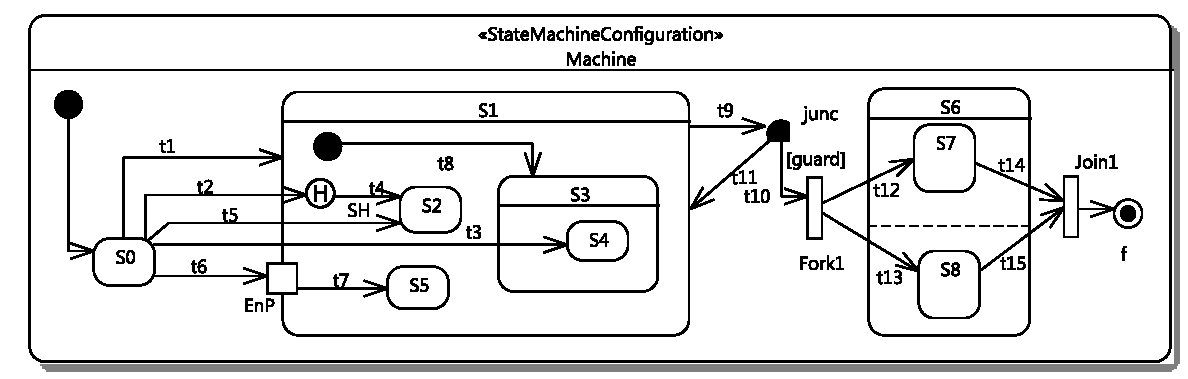
\includegraphics[clip, trim=0.2cm 0.2cm 0.2cm 0.2cm, width=1.0\columnwidth]{figures/EnteringStateExample.pdf}
	\caption{Example illustrating different ways entering a composite state} 
	\label{fig:entering}
\end{figure}

A region $r$ is entered by either a transition $t$ in the border of its containing state or in a sub-vertex, depending on how the state machine is designed. 
The following lists different ways $r$ may be entered:
\begin{itemize}
	\item Way 1: entering by default: $tgt(t) = ctner(r) \wedge src(t) \notin subvts(r)$.
	
	\item Way 2: entering on a direct sub-vertex: $tgt(t) \in subvts(r) \wedge src(t) \notin subvts(r)$.
	
	\item Way 3: entering on an indirect sub-vertex: $ctner(tgt(t)) \in subvts^+(r) \wedge src(t) \notin subvts(r)$.
\end{itemize} 

All of the entering ways execute the entry action of the containing composite state $entry(ctner(r))$ after $effect(t)$. \ti{doActivity(ctner(r))} is then signaled to be run in a waiting thread (see \ref{sec:thread} for thread-based concurrency). The action execution afterward is different from each way. To illustrate, we use an example as in Fig. \ref{fig:entering} with \ti{S1} as a target composite state. \ti{t1} and \ti{t3} are in the ways of 1 and 3, respectively, while \ti{t2, t5} in the way 2. 

The entering method associated with the region $r$ of \ti{S1} has a parameter $enter_mode$ indicating how actions should be executed. $enter_mode$ takes values depending the number of transitions coming to the composite state $S1$: $\#values(s) = \\ \#\{v \in subvts(s)| v.kind=initial\} + \\ \#\{v \in subvts(s)| \exists t \in T_{ins}(v), src(t) \notin subvts(s)\} + \\ 
\#\{v \in subvts^+(s)\setminus subvts(s)|\exists t \in T_{ins}(v), src(t) \notin subvts^+(s)\}$. In this case these values are $\{DEFAULT = 0, SH\_MODE = 1, S2\_MODE = 2, S4\_MODE=3\}$. Listing \ref{lst:region} shows the C++-like example code generated for $r$.

  

\begin{lstlisting}[caption=Example code generated for the region of S1, label=lst:region, frame=single]
void S1Region1Enter(int enter_mode){
if (enter_mode == DEFAULT) {
  states[S1_ID].actives[0] = S3_ID;
  states[S3_ID].entry();  sendStartSignal(S3_ID);
  S3Region1Enter(DEFAULT);
} else if (enter_mode == S2_MODE) { //entry
  states[S1_ID].actives[0] = S2_ID;
  states[S2_ID].entry();  sendStartSignal(S2_ID);
} if (enter_mode == SH_MODE) {
  StateIDEnum his;
  if (states[S1_ID].pres[0] != STATE_MAX){
    his = states[S1_ID].pres[0];
  } else {
    his = S2_ID;
  }
  states[S1_ID].actives[0] = his;
  states[his].entry();  sendStartSignal(his);
  if (S3_ID == his) {
    S3Region1Enter (S3_REGION1_DEFAULT);
  } 
} else if (enter_mode == S4_MODE) {
  states[S1_ID].actives[0] = S3_ID;
  states[S3_ID].entry();  sendStartSignal(S3_ID);
  S3Region1Enter(S4_MODE);
} else if (enter_mode == EXP_MODE) {...}
\end{lstlisting}

For each value in $values(s)$, the region of $S1$ is entered and executes different actions. By default, the active sub-state of the region is set before the execution of any effect associated with the initial transition starting from the pseudo initial state of the region. $S3$ is set as active sub-state of $S1$. Entering on a direct sub-state (\ti{S2}) sets the active sub-state of \ti{S1} directly to \ti{S2}. In case of an indirect sub-state ($S4$), the entry action of the sub-state ($S3$) of $S1$ is executed before $S4$ is set as the active-sub state of $S3$ and the execution of $entry(S4)$. It is worth noting that after the execution of each entry, a start signal is sent to activate the sleeping thread associated with \ti{doActivity} of the corresponding state (see \ref{subsubsec:thread} for thread-based concurrency design).

Transitioning from a vertex to another vertex (transition from $S0$ to $SH$ is a particular case) is not as simple as that of two states. It needs a systematic approach which generates code for a transition outgoing from a vertex to any other one. This is detailed in the next section.

\subsection{Event and transition transformation}
\label{subsec:event}
\subsubsection{Events}
An event enumeration \ti{EventId} is created whose children are event identifiers associated with events. Each event $e$) is also transformed into a method $mtd_e$ in the context class $C$. Suppose $levents$ is the list of events which can be processed by the state machine $sm$. Besides the explicitly defined events of the state machines, $levents$ contains a special event called $CompletionEvent$. The latter is, following the UML specification, an implicit event triggering triggerless transitions. It is emitted when either \ti{doActivity} of an atomic state finishes its execution or all regions of a composite state have reached to a final state. The other events are transformed as followings:

\begin{itemize}
	\item \ti{CallEvent} $ce$: The operation associated with $ce$ can be either synchronous or asynchronous. When the former is called, it waits and takes the main mutex protecting the run-to-completion semantics, and executes $mtd_{ce}$. Contrarily, the parameters of the asynchronous operation are used to create a signal which is transformed similarly to the case of $SignalEvent$.
	
	\item \ti{SignalEvent} $se$: $SignalEvent$ is asynchronous. 
	The signal associated with $se$ is written into the event queue of the active class $C$ by an operation which takes as input the signal. 
	
	\item \ti{TimeEvent} $te$: A thread $teThread$ associated with $te$ is created and initialized at the initialization of the state machine. 
	Within the execution of $teThread$, the method associated $te$ waits for a signal, which is sent after the execution of the entry of a state $s \in \{v \in V|\exists t \in T_{outs}(v), te \in events(t)\}$, to start sleeping for a duration $d$ associated with $te$. 
	At the completion of the sleeping, $te$ is emitted and written to the event queue if $s$ is still active.
	
	\item \ti{ChangeEvent} $che$: Similar to $TimeEvent$, a thread $cheThread$ is initialized at initialization but the associated method $mtd$ does not wait for a signal to start. $mtd$ periodically checks whether the value of the associated boolean expression $ex(che)$ changes by comparing the current value with the previous value. 
	If a change happen, $che$ is committed to the event queue.
	
	\item \ti{Any}: any of the above events can trigger the associated transitions.
\end{itemize}

$CompletionEvent$ has the highest priority. Others are equal by default but their priority is configurable.

\subsubsection{Transitions}

To process events, for each event, a method is implemented in $C$. Each event triggers a list of transitions. We suppose $T_{trig}(e)$ is the transition list triggered by the event $e$, and $S_{trig}(e) = \{src(t) | t \in T_{trig}(e)\}$. In other words, $S_{trig(e)}$ is a set of states which are the source states of the transitions in $T_{trig}(e)$. To present how the body of event methods is generated, we define functions as followings:
\begin{itemize}
	\item Vertex depth $dp(v)$ is defined as:
			\begin{equation}
			dp(v) =    \left\{
			\begin{array}{ll}
			1 & \ti{v is a root vertex}  \\
			dp(ctner(v)) + 1& otherwise \\
			\end{array} 
			\right.
			\end{equation}
	\item $Map_{e}(s) \subset S_{trig(e)} | \forall sub \in Map_e(s): ctner(sub) = s$, $Prt(e) = \{s \in V| Map_{e}(v) \neq \emptyset\}$. $Prt(e)$ is an ordered list whose length is $len(Prt\{e\})$ and elements are accessed by indexes. The order of $Prt(e)$ is defined as:	$\forall i, j \leq len(Prt\{e\})$, 
	\\ if $i < j, dp(Prt(e).get(i)) \geq dp(Prt(e).get(j))$. 	
\end{itemize}

\begin{lstlisting}[mathescape=true, caption=Generation process for an event, label=lst:eventproc, frame=single]
$\forall$ item $\in Lm(e)$
  $\forall s \in Map_e(item)$
    $T_s = \{t \in T_{trig}(e)|src(t) = s\}$
    $\forall t \in T_s$
	    $GENERATE\_STATE\_EVENT\_CHECK(s, t, e)$
	    $GENERATE\_GUARD(t)$
      $GENTRANS(s,t,tgt(t))$  	
\end{lstlisting}

The procedure in Listing \ref{lst:eventproc} describes how the generation process works with an event. 
It first finds the innermost active states which are able to react $e$ by orderly looping over $Lm_e$. 
For each transition outgoing from an innermost state, code for active states and deferral events, guard checking and transition code segments are generated by $GENERATE\_STATE\_EVENT\_CHECK$, $GENERATE\_GUARD(t)$ and \ti{GENTRANS}, respectively. 
If the identifier of $e$ is equal to one of the events listed in $defEvents$ of the corresponding state (not shown in this paper), it is deferred by putting it to a deferral event queue managed by the main thread, which also pushes the deferred events back to the main queue once one of the pending events is processed. 

Generally, \ti{GENTRANS} generates code for transitions between any vertexes satisfying the constraints described in Section \ref{subsec:background}. Algorithm \ref{alg:transitiongeneration} shows how the transition code generation works. The generated code is bounded by the deferral events, active states, and guard checking.

\begin{algorithm}[]
	\caption{Code generation for transition
		\label{alg:transitiongeneration}}
	\begin{algorithmic}[1]
		\Require{A source $v_{s}$, a target vertex $v_{t}$ and a transition $t$}
		\Ensure{Code generation for transition}
		\Procedure{genTrans}{$v_s$, $v_t$, $t$}
		\Let{$H_s$}{$v_s \cup ctner^+(v_s)$}
		\Let{$H_t$}{$v_t \cup ctner^+(v_t)$}
		\State {$s_{ex} \in H_s, s_{en} \in H_t | ctner(s_{ex}) = ctner(s_{en})$}
		%\Let{\{$s_{ex}, s_{en}$\}}{$FINDEXE(v_s, v_t)$}
		\State {//Generate IF-ELSE statements for junctions}
		\If {$s_{ex}$ is a state}
		\For {$ r \in regions(s_{ex})$}
		\State {$FORK(RegionExit(r))$}
		\EndFor
		\State {//Generate JOIN for threads created above}
		\State {//Generate sendStopSignal to $s_{ex}$}
		\State {$exit(s_{ex})$}	
		\EndIf
		\If {$v_t.kind=join$}
		\For {$in \in T_ins(v_t)$}
		\State {$FORK(effect(in))$}
		\EndFor
		\State {//Generate JOIN for threads created above}
		\Else
		\State {$effect(t)$}	
		\EndIf
		\If {$s_{en}$ is a state}
		\State {$entry(s_{en})$}
		\State {//Generate sendStartSignal to $s_{en}$}
		\If {$s_{en}.kind\in\{conp,conc\}$}
		\For {$ r \in regions(s_{en})$}
		\State {$FORK(RegionEnter(r))$}
		\EndFor
		\State {//Generate JOIN for threads created above}
		\EndIf
		\Else
		\State {//Generate for pseudo states by patterns}
		\EndIf
		\EndProcedure	
	\end{algorithmic}
\end{algorithm}

In the first place, Algorithm \ref{alg:transitiongeneration} looks for the composite states $s_{ex}$ and $s_{en}$ at the highest level to be exited and entered, respectively, by using Algorithm \ref{alg:findexit-entry} (line 2-4). 
If the transition $t$ is part of a compound transition, which involves some $junction$s, IF-ELSE statements are generated first (as PSCS says $junction$ is evaluated before any action), as described by the following list. 
The composite state is exited by calling the associated exiting region methods (FORK and JOIN for orthogonal regions)and followed by the generated code of transition effects. Entering region methods are then called once the above code completes the execution. If the target $v_t$ of the transition $t$ is a pseudo state, the generation algorithm corresponding to the pseudo state type is called. These algorithms are shown as the below list. 
 

%It generates the code checking for active states respecting the UML semantics in which the innermost states process the incoming event first. To do this, it first looks in the source state list $S_{trig(e)}$ for the innermost states that accept the event triggering its outgoing transitions. If these found states are children of a concurrent state, $genStateCheck$ generates the checking codes run in parallel, which will be described later in \ref{subsubsec:thread}. Otherwise said, sequential code is generated.


\begin{comment}



\begin{algorithm}[]
	\caption{Find states should be exited and entered
		\label{alg:findexit-entry}}
	\begin{algorithmic}[1]
		\Require{A source $v_{s}$ and a target vertex $v_{t}$}
		\Ensure{Vertexes $s_{ex}$, $s_{en}$ to be exited, and entered, respectively}
		\Procedure{findExE}{$v_s$, $v_t$}
			\Let{$H_s$}{$v_s \cup ctner^+(v_s)$}
			\Let{$H_t$}{$v_t \cup ctner^+(v_t)$}
			\State {$s_{ex} \in H_s, s_{en} \in H_t | ctner(s_{ex}) = ctner(s_{en})$}
		\EndProcedure	
	\end{algorithmic}
\end{algorithm}
\end{comment}

\begin{itemize}
	\item $join$: Use $GENTRANS$ for $v$'s outgoing transition.
	
	\item $fork$: Use $FORK$ and $JOIN$ for each of outgoing transitions of $v$.
	
	\item $choice$: For each outgoing, an $IF-ELSE$ is generated for the guard of the outgoing together with code generated by $GENTRANS$ (see Listing \ref{lst:event1}).
	
	\item $junction$: As a static version $choice$, a $junction$ is transformed into an attribute $junc_attr$ and evaluated before any action executed in compound transitions (see Listing \ref{lst:event1}). 
	The value of $junc_attr$ is then used to choose the appropriate transition at the place of $junction$.
	
	\item \ti{shallow history}: The identifiers of states to be exited are kept in $pres$ of $IState$. Restoring the active states using the history is exampled as in Listing \ref{lst:region}. The entering method is executed as default mode at the first time the corresponding composite state is entered (see Listing \ref{lst:region}).
	
	\item \ti{deep history}: Saving and restoring active states are done at all state hierarchy levels from the composite state containing the deep history down to atomic states.
	
	\item $enpoint$: If $enpoint$ has no outgoing transition, the corresponding composite state is entered by default. Otherwise said, $GENTRANS$ is called to generate code for the outgoing transition.
	
	\item $expoint$: The code for the unique transition outgoing from $expoint$ is generated by using $GENTRANS$.
	
	\item $terminate$: The code executes the exit action of the innermost active state, the effect of the transition and destroys the state machine object.
\end{itemize}

\subsubsection{Example Code} Listing \ref{lst:event} shows a code segment generated for the processing of the event $verifyingPIN$. It first checks whether $Idle$ is the current active state, in which $activeStateID$ is the identifier of the current root active state. The $doActivity$ behavior of $Idle$ is then stopped upon receiving a stop signal (line 2). The effect of $t2$ is executed after the execution of $exit(Idle)$ (line 3-4). $effect(t3)$ and $effect(t4)$ are then concurrently executed by using $FORK$ and $JOIN$ (line 5-8) since the owning transitions outgo from a $fork$. The execution of $emtry(Verifying)$ (line 11) then follows the changing the root active state to $Verifying$ (line 10). $doActivity(Verifying)$ is triggered in its own thread upon receiving a start signal (line 11) followed by concurrently entering the two orthogonal regions of $Verifying$ with appropriate modes.

 
\begin{lstlisting}[caption=Example code generated for event $verifyingPIN$, label=lst:event, language=C++]
if (activeStateID == IDLE_ID) {
  sendStopSignal(IDLE_ID);  exit_Idle();
  effect_t2();
  thread_t3 = FORK(effect_t3);  thread_t4 = FORK(effect_t4);
  JOIN(thread_t3);  JOIN(thread_t4);
  activeStateID = VERIFYING_ID;  entry_Verifying();
  sendStartSignal(VERIFYING_ID);
  th_r1 = FORK(R1Enter(VERIFYINGCARD_MODE));
  th_r2 = FORK(R2Enter(VERIFYINGPIN_MODE));
  JOIN(th_r1);  JOIN(th_r2);
}
\end{lstlisting}


\begin{lstlisting}[caption=Example code generated for $Join1$ and $Junction1$, label=lst:event1, language=C++]
if((states[VERIFYING_ID].actives[0]==CARDVALID_ID)
&&(states[VERIFYING_ID].actives[1]==PININCORRECT_ID)) {
	Junction1 = 0; //else outgoing transition of Junction1
	if (tries < maxTries) {Junction1 = 1;}
	FORK(R1Exit); FORK(R2Exit);
	//JOIN ...
	sendStopSignal(VERIFYING_ID);	exit(VERIFYING_ID);
	FORK(effect_t11); FORK(effect_t13);
	//JOIN ...
	if (Junction1=1) {
		tries++;
		activeStateID = IDLE_ID;		entry(IDLE_ID);
		sendStartSignal(IDLE_ID);
	} else {
		cardValid = false;
		activeStateID = IDLE_ID;		sendStartSignal(IDLE_ID);
	}
}
\end{lstlisting}



 


 

